\section{Instruction Selection}

\subsection{Tree Patterns}
在 intermediate representation (Tree) language 中, 一个操作用一个树节点表示. 一条机械指令需要执行一些基本操作, 可以用 IR tree 的一个片段表示, 称为 tree pattern(树模式). 指令选择的任务就是使用树模式的最小集合来覆盖 (tile).

使用 Jouette 体系, 将树模式映射为指令, 如 \ref{fig:Jouette} 所示.

一棵树可以有多种覆盖方式. 

\subsubsection{Optimal and Optimum Tilings}
\begin{itemize}
    \item optimum tiling (最优覆盖): 覆盖的代价和是最小的覆盖,全局最优.
    \item optimal tiling (最佳覆盖): 不存在两个相邻的覆盖能连接成一个代价更小的覆盖,局部最优.
\end{itemize}
全局最优属于局部最优.

\begin{figure}[H]
    \centering
    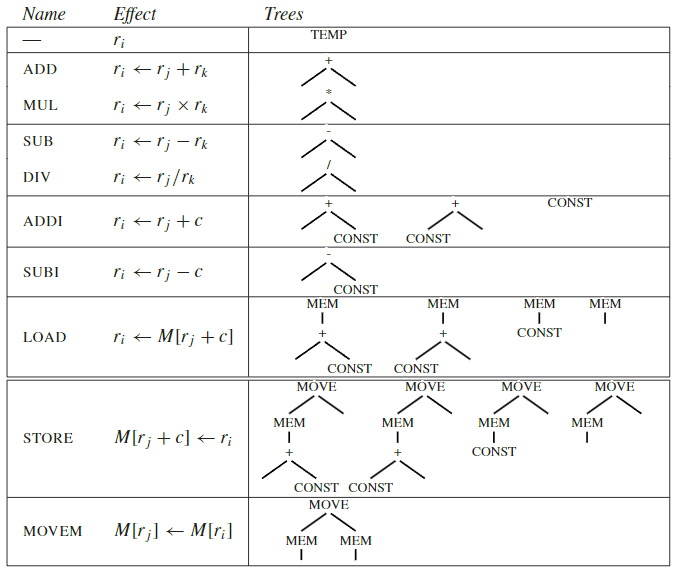
\includegraphics[width=0.94\linewidth]{pic/CP9/Jouette architecture}
    \caption{Jouette architecture}
    \label{fig:Jouette}
\end{figure}

\subsection{Algorithm for Instruction Selection}
\subsubsection{Maximal Munch}
最佳覆盖的算法.

从树的根节点开始寻找 适 合 他 的 最 大 覆盖 (覆盖的节点数最多, 如果相等的可以任意选择其一), 按 照 Jouette 体系结构可能会覆盖其他几个节点; 对遗留的其他 子 树 也 进 行 相 同 操 作.

Maximal Munch 算 法 的 tiling 是从顶向下的,但是指令的生成是逆序的(很好理解,因为上层的覆盖指令需要下层的指令提供操作数,所以是逆序).


\subsubsection{Dynamic Programming}
可以找到最优覆 盖 , 子 问 题 是 子 树 的 覆 盖, 自下而上工作.

会给每个节点计算一个代价, 表示可以覆盖该节点为根的子树的指令序列最优的代价之和. 

对于一个节点 $n$, 先找到其所有子树的代价 $c_i$, 然后枚举节点 $n$ 所有可能的覆盖, 计算每种覆盖的代价 $c+\sum c_i$, 最后选择代价最小的覆盖.

不同的覆盖代价不同, 具体的代价书中没有给出, 看着默认都是 1, 即目标是覆盖的数量最少.

\subsubsection{Tree Grammar(树文法)}
DP 的推广. 使用 brain-damaged Jouette 体系.

使用 CFG 来描述覆盖,文法具有高 度歧义性, 但是 DP 可以很好 处理给出最优的覆盖.

\begin{figure}[H]
    \centering
    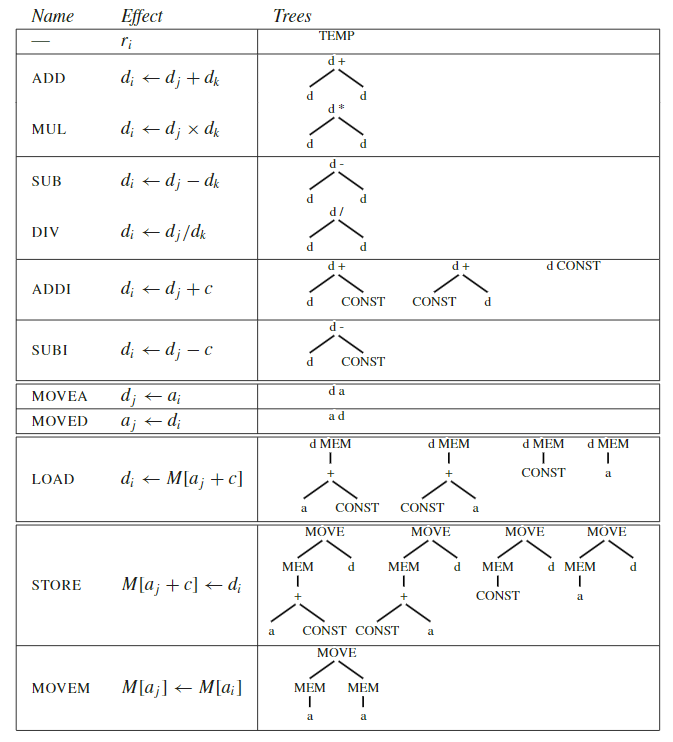
\includegraphics[width=0.94\linewidth]{pic/CP9/The Schizo-Jouette architecture}
    \caption{The Schizo-Jouette architecture}
\end{figure}


有两类寄存器:
\begin{itemize}
    \item a 寄存器:存地址;
    \item d 寄存器:存数据
\end{itemize}

\begin{figure}[H]
    \centering
    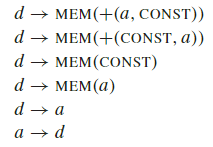
\includegraphics[width=0.32\linewidth]{pic/CP9/The grammar rules}
    \caption{The grammar rules for the LOAD , MOVEA and MOVED instructions}
\end{figure}


\subsubsection{Efficiency of Tiling Algorithms}
$T$ 个覆盖,平均每个匹配的覆盖有 $K$ 个非叶子节点. $K'$ 是在给定子树中为确定匹配那个覆盖需要检查的最大节点个数(近似于最大覆盖的大小). 假定平均每个树节点可以与 $T'$ 个覆盖匹配. 输入树的节点为 $N$.
\begin{itemize}
    \item Maximal Munch: 平均只需要遍历 $N/K$ 个节点, 就可以覆盖整棵树, 所以 复杂度为 $O((K'+T')N/K)$
    \item DP: 需要遍历所有节点的所有覆盖可能, 复杂度为 $O((K'+T')N)$
\end{itemize}
DP 的其他常数也比 Maximal 大, 因为要遍历两遍. $K',K,T$ 是常数, 线性复杂度.

\subsection{CISC Machines}
RISC(Reduced Instruction Set Computer) 机器特征:
\begin{enumerate}
    \item 32 个寄存器
    \item 仅有一类整数/指针寄存器
    \item 算数运算仅对寄存器进行操作
    \item 采用``三地址''指令$(r_1\leftarrow r_1+r_2)$
    \item 取指令和村指令只有 M[reg+const]模式
    \item 每条指令长度固定为32 位
    \item 每一条指令产生一个结果或作用,无副作用
\end{enumerate}

CISC(Complex Instruction Set Computer) 机器特征:
\begin{enumerate}
    \item 不多的几个寄存器(16,8,6)
    \item 寄存器分不同类型,某些操作只能在特定种类的寄存器上进行
    \item 算术运算可以通过不同的寻址模式访问寄存器和储存器
    \item 指令是``两地址''指令
    \item 有不同的寻址模式
    \item 有由变长操作码加变长寻址模式形成的变长指令
    \item 指令具有副作用(自增寻址方式)
\end{enumerate}

CISC 机器的特点解决难题:
\begin{enumerate}
    \item  寄 存 器 较 少 : 不 限 制 生 成TEMP 节点,假设寄存器分配能完成分配工作
    \item 寄存器分类:将操作数显示地传送到相应的寄存器中
    \item 两地址指令:增加一条额外的传送指令
    \item 算数运算可以访问存储器:指令选择阶段将每一个 TEMP 节点转化成一个寄存器引用.
    \item 若干种寻址模式:优点(破坏寄存器少;指令代码短)
    \item 变长指令:不管;
    \item 副作用指令
\end{enumerate}

三种解决办法:
\begin{enumerate}
    \item 忽略地址自增指令,希望其自动消失
    \item 在采取树型匹配的代码生成器的上下文中使用特别方式匹配特殊的习惯用法
    \item 使用完全不同的指令算法,基于 DAG 样式.
\end{enumerate}